\normaltrue \difficilefalse \tdifficilefalse
\correctionfalse

%\UPSTIidClasse{11} % 11 sup, 12 spé
%\newcommand{\UPSTIidClasse}{11}

\exer{Représentation 2D$\star$ \label{E2:05:1016}}
\setcounter{question}{0}\marginnote{\xpComp{PPM}{01}}%\UPSTIcompetence[2]{E2-05}
\index{Compétence E3-05}\index{Compétence PPM-01}
\index{Représentation 2D}

\ifcorrection
\else
\marginnote{\textbf{Pas de corrigé pour cet exercice.}}
\fi


\ifprof 
\else
Soit la pièce suivante.
\begin{center}
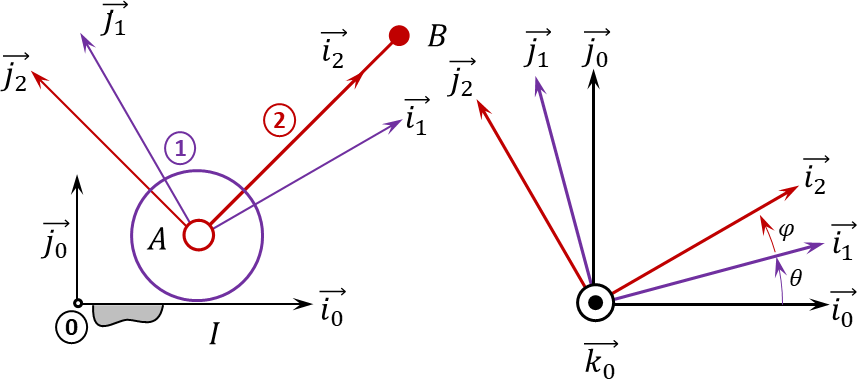
\includegraphics[width=.7\linewidth]{01}
\end{center}
 \fi
 
\question{Compléter les vues suivantes.}
\ifprof
\begin{marginfigure}
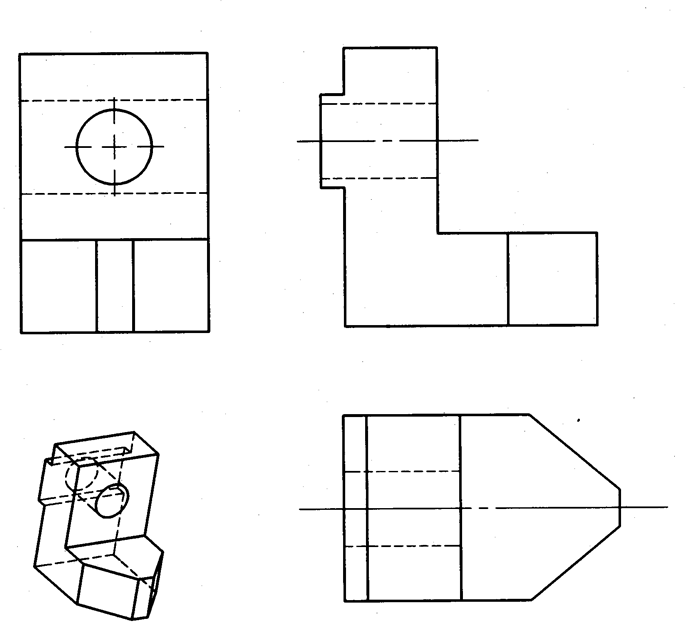
\includegraphics[width=\linewidth]{01_cor}

\includegraphics[width=\linewidth]{02_cor}
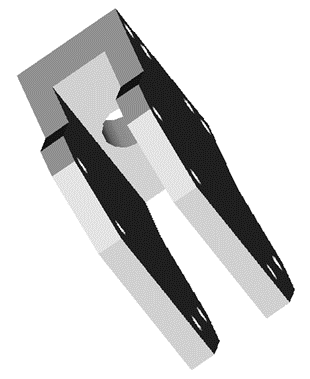
\includegraphics[width=\linewidth]{03_cor}
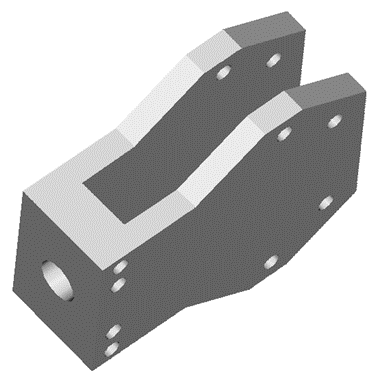
\includegraphics[width=\linewidth]{04_cor}
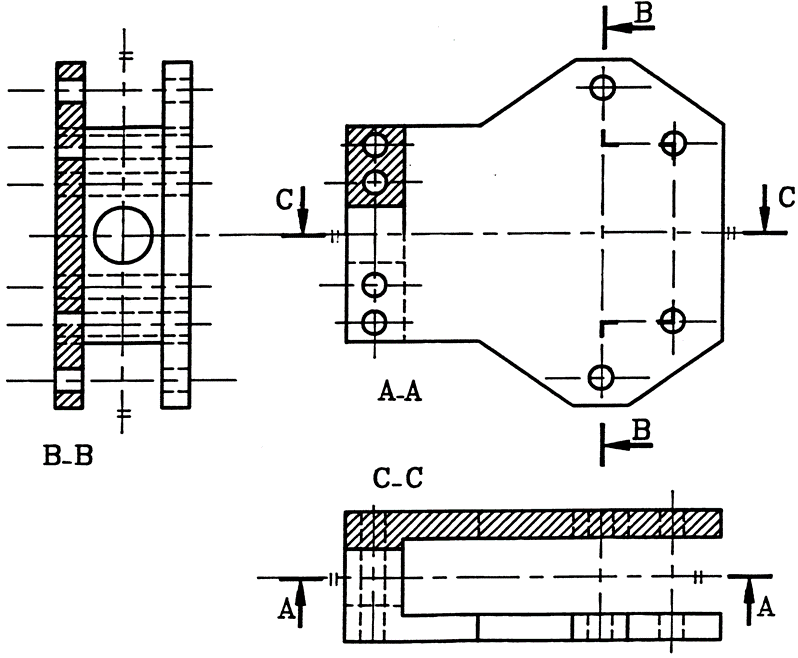
\includegraphics[width=\linewidth]{05_cor}
\end{marginfigure}
\else 
\begin{marginfigure}
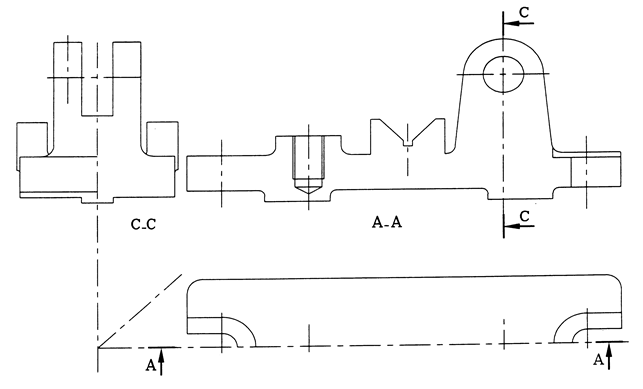
\includegraphics[width=\linewidth]{02}
\end{marginfigure}
\fi

\ifprof
\else

\marginnote{Corrigé voir \ref{E2:05:1016}.}

\fi